\section{Motivation}
\label{sec:motivation}


In this section we motivate our runtime-assisted approach to
convergent RDTs with help of a set data structure.

\begin{figure}[ht]
\centering
\begin{ocaml}
module Set: sig
  type t (* Abstract type of the set*)    
  type elt (* Abstract type of set elements *)
  val add: elt -> unit (*Add an element *)
  val remove: elt -> unit (* Remove an element *)
end
\end{ocaml}
\caption{An OCaml interface to \C{Set} abstract data type.}
\label{fig:ocaml-set}
\end{figure}

\begin{figure}[ht]
  \centering
  \begin{subfigure}[t]{0.55\columnwidth}
    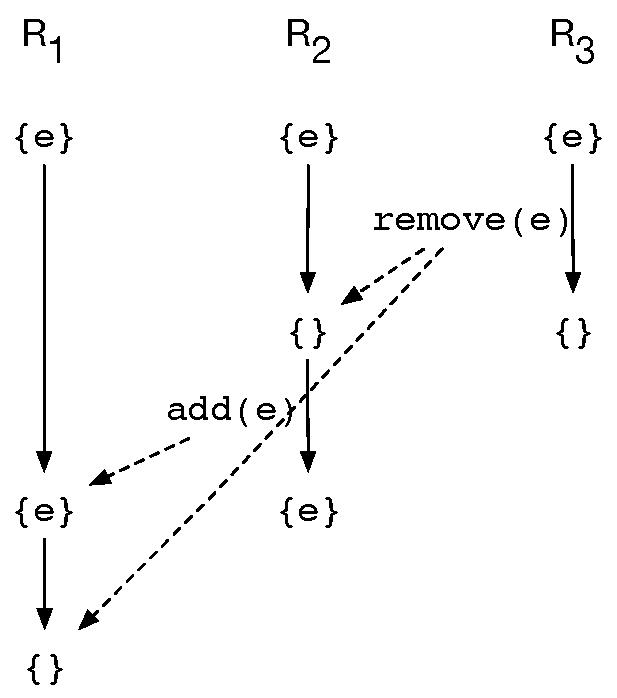
\includegraphics[scale=0.35]{Figures/crdt-execs-1}
    \caption{}
    \label{fig:crdt-exec-1}
  \end{subfigure}
  \begin{subfigure}[t]{0.44\columnwidth}
    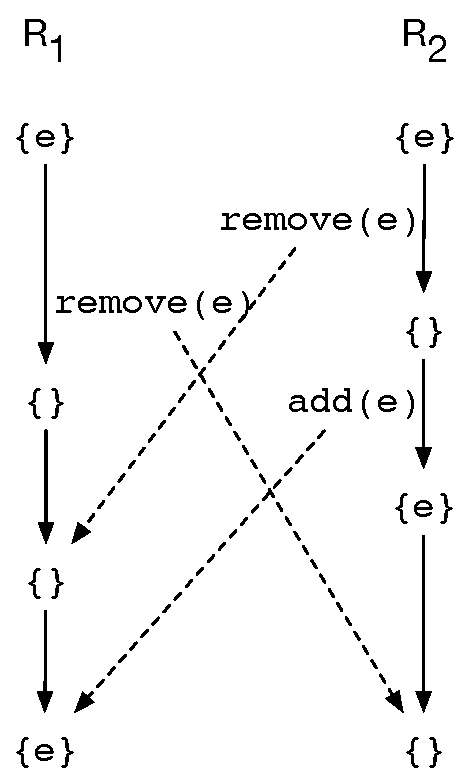
\includegraphics[scale=0.35]{Figures/crdt-execs-2}
    \caption{}
    \label{fig:crdt-exec-2}
  \end{subfigure}
\caption{Anamolous executions from asynchronous
  replication of \C{Set}. Dashed lines denote effect propagation.}
\label{fig:crdt-execs}
\end{figure}

\noindent\paragraph{From Set ADT to Set RDT} Fig.~\ref{fig:ocaml-set}
shows a simplified interface of \C{Set} (abstract) data type in OCaml.
The interface hides a reference to a set (\C{Set.t}), which can be
updated in-place via \C{add} and \C{remove} operations. \C{Set} is an
ordinary data type meant for sequential execution. Under a
concurrent execution with an asynchronously replicated state, \C{Set}
would exhibit anamolous behaviors such as those in
Fig.~\ref{fig:crdt-execs}.

Fig.~\ref{fig:crdt-exec-1} shows an anamolous execution with three
replicas -- $R_1$, $R_2$, and $R_3$, all of which start with a
singleton set containing the element $e$. A client connects to the
replica $R_3$ and executes a \C{remove($e$)} operation, which is then
asynchronously propagated to other replicas. Some time after applying
$R_3$'s \C{remove} at $R_2$, another client connects to $R_2$ and
re-adds $e$ by issuing an \C{add($e$)} operation. Consequently, the
state at $R_2$ is again the singleton set $\{e\}$. Replica $R_3$
however receives $R_2$'s \C{add} ahead of $R_1$'s \C{remove}, applies
them in the same order, and ends up with an empty set. The execution
thus results in divergent replica states.

Note that if \C{Set.add} and \C{Set.remove} commute, then executing
them in different order at $R_2$ and $R_3$ would not have led to
divergence. As such, \C{Set} is not a CRDT due to the admittance of
non-commutative operations. Nonetheless, there exist approaches to
transform \C{Set} into a CRDT by re-engineering its interface and
operations~\cite{crdts, zawirski-thesis, zhang}. For instance, the
anomalous execution in Fig.~\ref{fig:crdt-exec-1} can be preempted
by ensuring that updates are only ever applied in the causal order.
This can be done by extending \C{Set} with vector clocks to keep track
of the causal history of each operation. A set \C{add} (resp.
\C{remove}) would now generate an \C{Add} (resp.  \C{Remove})
\emph{effect} tagged with the vector clock of the origin replica.
Here, the vector clock simply records the sequence number of last
operation from each replica whose effect has been received and applied
at the current replica. When an effect is received at a replica, it is
buffered until the time all its causally-preceding effects (as
captured by the tagged vector clock) have already been received and
applied. This strategy would preempt the execution in
Fig.~\ref{fig:crdt-exec-1} by buffering $R_2$'s \C{add} at $R_1$
until the causally-preceding \C{remove} of $R_1$ is received and
applied. An interface for such a \emph{causally-consistent} set RDT is
shown in Fig.~\ref{fig:cc-set}. 

\begin{figure}[ht]
\centering
\begin{ocaml}
module Set: sig
  type t      type elt
  type r_id (* Replica Id *)
  (* Vector Clock *)
  type v_clock = (r_id,int) HashTable.t 
  (* Set RDT Effects *)
  type eff = Add of elt * v_clock 
           | Remove of elt * v_clock
  (* This replica's vector clock *)
  val local_clock: v_clock 
  val add: elt -> eff
  val remove: elt -> eff
  val buf: eff list (* pending effects *)
  (* Apply an effect to the local state *)
  val apply_eff: eff -> unit
end
\end{ocaml}
\caption{An OCaml interface to \C{Set} replicated data type}
\label{fig:cc-set}
\end{figure}

\noindent\paragraph{Add-Wins Set CRDT} Unfortunately, \C{Set}
data type of Fig.~\ref{fig:cc-set} still admits divergent executions
due to concurrent updates.  Fig.~\ref{fig:crdt-exec-2} describes one
such execution. Here, replicas $R_1$ and $R_2$ both start with a
singleton set $\{e\}$.  Two distinct clients connect to $R_1$ and
$R_2$ respectively and issue two concurrent \C{remove($e$)}
operations. Later, another client connects to $R_2$ and issues an
\C{add($e$)} operation. The effects of these operations are
asynchronously applied at remote replicas as shown in the figure,
causing divergent states at $R_1$ and $R_2$.

Note that, unlike the execution in Fig.~\ref{fig:crdt-exec-1}, the
conflicting operations in Fig.~\ref{fig:crdt-exec-2}, namely $R_1$'s
\C{remove} and $R_2$'s \C{add}, are \emph{not} causally related,
hence their relative order is not determined by the sequential
specification of the data type. Forcing a causal relationship between
them requires synchronization between \C{add}s and \C{remove}s,
which is expensive in an asynchronous distributed setting. It
therefore becomes inevitable to ascribe semantics to concurrent
executions to restore convergence. This is done by imposing an
\emph{arbitration order} among concurrent conflicting operations,
which are otherwise unordered. For example, in
Fig.~\ref{fig:crdt-exec-2}, we might let $R_2$'s \C{add} override
$R_1$'s \C{remove} considering that \C{add} is re-adding an
element after a previous remove. Ordering concurrent removes ahead
of adds uniformly on all replicas leads to an implementation of
\C{Set} RDT where concurrent (re-)adds consistently \emph{win}
over removes. Such an \emph{add-wins} set is useful, for instance, in
an online shopping cart where two users can concurrently
remove an item, but if one of them re-adds it, then the
item is present in the final cart\footnote{This is in fact the
semantics of Amazon's online shopping cart~\cite{dynamo}.}.

Extending the \C{Set} implementation from Fig.~\ref{fig:cc-set} with
\emph{add-wins} semantics is however not trivial. The suggested
approach involves tracking element-wise causal dependencies between
the \C{remove}s and \C{add}s by maintaining a vector clock \emph{for
each element} $e$ in the set~\cite{zawirski-thesis}. The vector clock
of $e$ records the sequence number of the last \C{add($e$)} operation
from each replica whose effect has been received and applied at the
current replica. The \C{Add} and \C{Remove} effects on $e$ will now be
tagged with $e$'s vector clock. When a \C{Remove} effect on $e$ is
received at a replica, it is applied only if the tagged vector clock
is no less than $e$'s local vector clock, i.e., only if the arriving
\C{Remove} has seen (i.e., causally succeeds) at least those
\C{add($e$)} operations the current replica is aware of.  Otherwise
the effect is simply a no-op. This strategy would result in convergent
states despite the execution in Fig.~\ref{fig:crdt-exec-2} as $R_2$'s
\C{remove} effectively becomes a no-op at $R_1$ due to there being at
least one \C{add} operation on $e$ that it hasn't seen. The
\emph{add-wins} \C{Set} interface is similar to Fig.~\ref{fig:cc-set},
except that it requires an additional data structure for
element-wise vector clocks: 
\begin{ocaml}
  val e_clock: (elt, v_clock) HashTable.t
\end{ocaml}
The resultant set RDT is assumed to be correct albeit a formal proof
of convergence could not be found in the literature. 

\noindent\paragraph{The problem with the CRDT approach} The above
exercise demonstrates the considerable ingenuity and effort involved
in deriving a convergent RDT out of such simple data type as \C{Set}.
Such sophistication makes it quite hard for non-expert developers to
build, or even customize existing replicated data types to suit the
needs of their application. Some of the effort can be mitigated by
strengthening the underlying system model insofar as it doesn't affect
the latency and availability of the application. For instance, a
system that always delivers messages in the causal order would
automatically preempt the execution in Fig.~\ref{fig:crdt-exec-1}
without the need for additional intervention on behalf of the
developer. This is a particularly attractive proposition considering
that causal consistency can be ``bolted on'' an existing
implementation of an eventually consistent system without weakening
its guarantees~\cite{BoltOn}. Unfortunately, such strengthening of the
system model would deliver no benefits to the developer if they still
have to reason about fine-grained causal dependencies to guarantee
convergence, such as in the case of Fig.~\ref{fig:crdt-exec-2}. As we
observed earlier, the execution in Fig.~\ref{fig:crdt-exec-2} seems
inevitable unless every pair of \C{add} and \C{remove} operations are
synchronized, which, regrettably, is not a practical option. The
developer therefore seems to be stuck.

\begin{figure}[ht]
  \centering
  \begin{subfigure}[t]{0.55\columnwidth}
    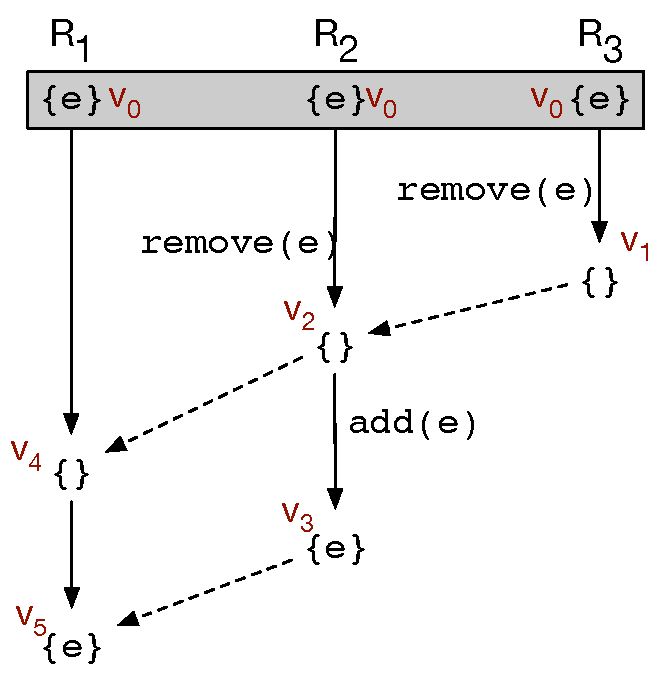
\includegraphics[scale=0.35]{Figures/mrdt-execs-1}
    \caption{}
    \label{fig:mrdt-exec-1}
  \end{subfigure}
  \begin{subfigure}[t]{0.44\columnwidth}
    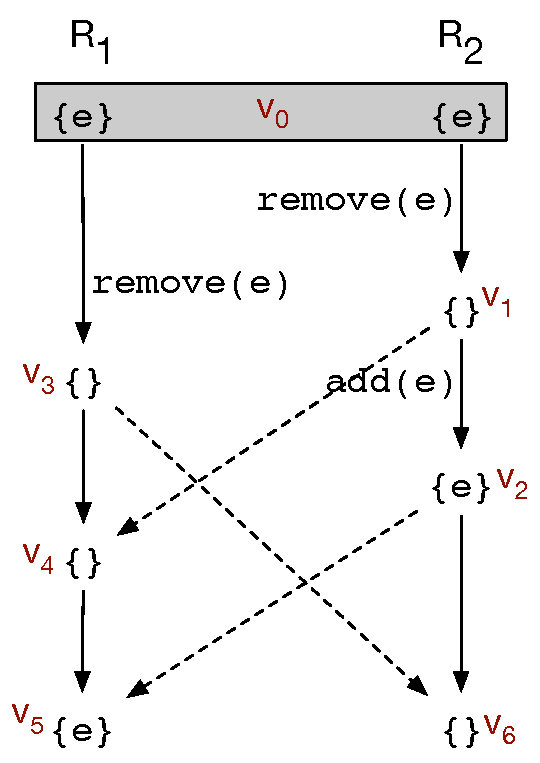
\includegraphics[scale=0.35]{Figures/mrdt-execs-2}
    \caption{}
    \label{fig:mrdt-exec-2}
  \end{subfigure}
\caption{Equivalent executions of Fig.~\ref{fig:crdt-execs} in
state-centric replication model. Dashed lines now denote state merges.}
\label{fig:mrdt-execs}
\end{figure}

\noindent\paragraph{The MRDT Approach} Mergeable Replicated Data Types
(MRDTs) implement a state-centric model of replication that is
inspired by the Git version control system. Like in Git, the state
evolves in terms of versions, and concurrent versions of the state can
be merged. The semantics of merge depends on the type of the state, so
each MRDT is required to be equipped with a three-way \C{merge}
function that merges concurrent versions of that type in presence of
their (lowest) common ancestor version. In our running example, the
state is a value of type \C{Set.t}, hence \C{Set.merge} would
have the signature:
\begin{center}
\C{Set.merge} : \C{Set.t} $\rightarrow$ \C{Set.t} $\rightarrow$ \C{Set.t}
$\rightarrow$ \C{Set.t}
\end{center}
The three arguments of \C{merge} correspond to the lowest common
ancestor (LCA) version and the two concurrent versions that
independently evolved from the LCA version. The LCA is a causal
ancestor of concurrent versions, hence causal consistency is built
into the replication model. The result of set merge, intuitively, must
contain the common elements in the two concurrent versions along with
any newly added elements in either versions. Concretely:
\begin{ocaml}
  let merge s(*lca*) s1 s2 = 
              (s1 $\cap$ s2) $\cup$ (s1 - s) $\cup$ (s2 - s)
\end{ocaml}
Extending \C{Set} ADT with the above merge function results in a
\C{Set} MRDT.

Let us now reconsider the executions in Fig.~\ref{fig:crdt-execs},
this time on \C{Set} MRDT. The equivalent executions are shown in
Fig.~\ref{fig:mrdt-execs}. Due to causal consistency being built into
the model, the divergent execution of Fig.~\ref{fig:crdt-exec-1} is
preempted in favor of the convergent execution shown in
Fig.~\ref{fig:mrdt-exec-1}. The execution manifests as follows.  The
initial version ($v_0$) on all three replicas  is the singleton set
$\{e\}$. Applying operations to replicas creates new versions, e.g.,
$v_1$ on $R_3$, and $v_2$ and $v_3$ on $R_2$. Changes can be
propagated by merging versions, e.g., version $v_2$ on $R_2$ is a
result of merging $v_1$ into $v_0$ for which $v_0$ serves as the
lowest common ancestor (LCA)
  \footnote{Versions $v_0$ and $v_1$ are not concurrent as the
  former is an ancestor of the latter. Merging $v_1$ into $v_0$ is
  nonetheless possible as $v_1$ is ahead of $v_0$ in causal order. In
  Git parlance this is a \emph{fast forward} merge.}.
Likewise $v_4$ on $R_1$ is created by merging $v_2$ into $v_0$ in
presence of their LCA $v_0$. The next version $v_5$ on $R_1$ is the
result of merging $R_2$'s $v_3$ into $R_1$'s $v_4$. The LCA for this
merge is $v_2$. By the end of the execution, versions $v_5$ and $v_3$
on $R_1$ and $R_2$ (resp.) have witnessed the same set of operations,
hence are in agreement.


\begin{figure}[ht]
  \centering
  \begin{subfigure}[t]{0.4\columnwidth}
    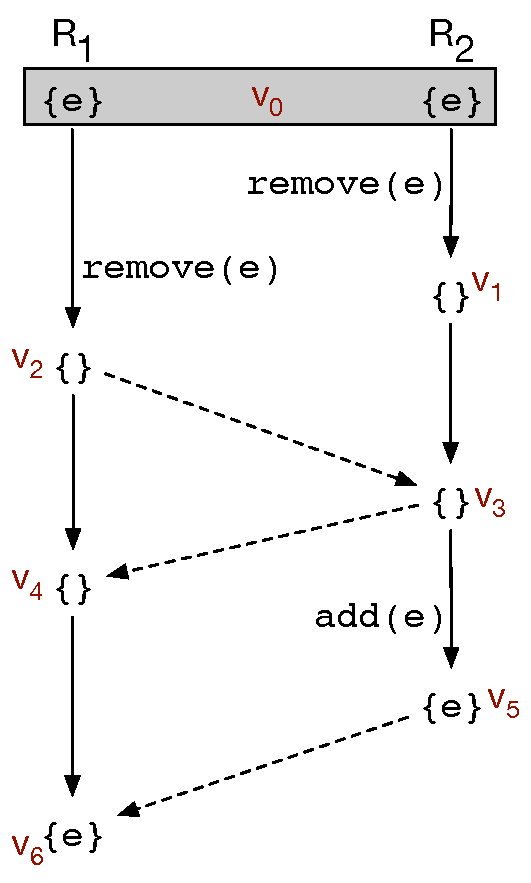
\includegraphics[scale=0.35]{Figures/mrdt-execs-3}
    \caption{}
    \label{fig:mrdt-exec-3}
  \end{subfigure}
  \begin{subfigure}[t]{0.57\columnwidth}
    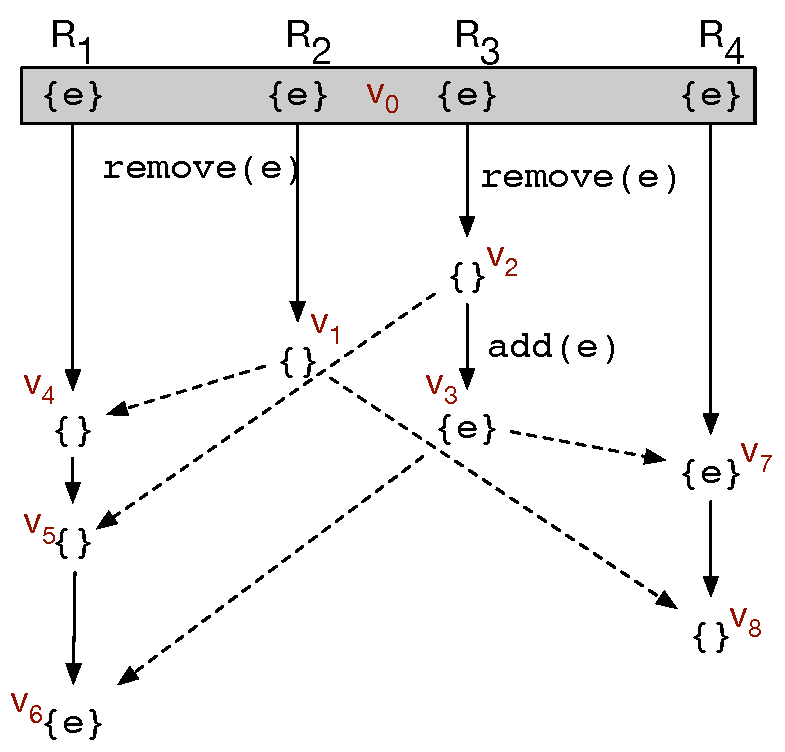
\includegraphics[scale=0.35]{Figures/mrdt-execs-4}
    \caption{}
    \label{fig:mrdt-exec-4}
  \end{subfigure}
  \caption{Executions demonstrating the difference between linearized
  (former) and concurrent (latter) merges.}
\label{fig:mrdt-execs-2}
\vspace*{-0.25in}
\end{figure}

\noindent\paragraph{Well-formed executions and the \quark runtime}
Convergence however is not an inherent virtue of the state-centric
replication model. Fig.~\ref{fig:mrdt-exec-2} shows the state-centric
analogue of the execution in Fig.~\ref{fig:crdt-exec-2} which
diverges. Here $R_1$ and $R_2$ start with version $v_0 \,=\, \{e\}$.
$R_2$ performs a \C{remove} and an \C{add} making versions
$v_1$ and $v_2$ respectively. Simultaneously, $R_1$ performs a
\C{remove} to make $v_3$. Replica $R_1$ now obtains $R_2$'s changes by
merging versions $v_1$ and $v_2$ to make new versions $v_4$ and $v_5$
respectively. LCAs for these merges are $v_0$ and $v_1$. Concurrently,
$R_2$ obtains $R_1$'s changes by merging $v_3$ with $v_2$ (LCA =
$v_0$) to make $v_6$.  Now $R_1$ and $R_2$ have same set of changes
yet their final versions differ.

Note that the anamolous execution in Fig.~\ref{fig:mrdt-exec-2} could
have been avoided had the merges between $R_1$ and $R_2$ been
linearized. Fig.~\ref{fig:mrdt-exec-3} shows an execution that only
slightly differs from the one in Fig.~\ref{fig:mrdt-exec-2}. The
difference is that the merges in Fig.~\ref{fig:mrdt-exec-3} happen
linearly: first $R_1$ is merged into $R_2$ (bringing $R_1$'s
\C{remove}), then $R_2$ into $R_1$ (bringing $R_2$'s \C{remove}),
followed again by $R_2$ into $R_1$ (bringing $R_2$'s \C{add}). As a
result of such linearization, the final versions on $R_1$ and $R_2$
converge to the singleton set $\{e\}$. Note that there exist other
linearizations of merges; for instance, $R_1 \,\rightarrow\, R_2$
merge could be ordered between the two $R_2 \rightarrow R_1$ merges.
However, all linearizations result in the same final state $\{e\}$.
Another important point to note is that only the merges are
linearized; not the entire execution. In Fig.~\ref{fig:mrdt-exec-3},
both $R_1$ and $R_2$'s \C{remove}s remove the same element $e$, which
is not possible in a linearized execution. %Leaving the execution
%unconstrained is crucial to satisfy the limits imposed by the CAP
%theorem on a highly-available partition-tolerant distributed system.

In the context of Fig.~\ref{fig:mrdt-exec-3}, it is quite clear what
linearization of merges means and how to enforce it via
synchronization (for e.g., wrapping each merge within a global lock).
In general however, the semantics of merge linearization isn't as cut
and dried. For instance, consider the execution in
Fig.~\ref{fig:mrdt-exec-4}. The four replicas involved in the
execution start with version $v_0 \,=\, \{e\}$. The replicas perform
local operations as shown in the figure to make versions $v_1$ to
$v_3$. Next they perform a series of merges to propagate local
changes. The merges can be ordered in time as following: first $R_2
\rightarrow R_1$ (merging $v_1$), then $R_3 \rightarrow R_1$ twice
(merging $v_2$ and $v_3$ resp.), then $R_3 \rightarrow R_4$ (merging
$v_3)$, and finally $R_2 \rightarrow R_4$ (merging $v_1$). These
merges collectively propagate the effects of \C{add} and \C{remove}
operations to $R_1$ and $R_4$. And despite being ordered in time,
they nonetheless result in a divergent execution ($v_6 \neq v_8$). The
problem here is that, although merges are executed linearly, the
execution graph does not reflect this linearity; merges that end in
$R_1$ in Fig.~\ref{fig:mrdt-exec-4} are effectively concurrent with
those that end in $R_4$. This shows that simply synchronizing the
execution of merges does \emph{not} result in convergence.

Our key insight to overcome this impasse is a novel \emph{well-formedness}
condition on execution graphs that ensures convergence of final
states. To understand well-formedness, let us contrast the bad
executions in Figs.~\ref{fig:mrdt-exec-2} and~\ref{fig:mrdt-exec-4}
against the good execution in Fig.~\ref{fig:mrdt-exec-3}. Observe that
in Fig.~\ref{fig:mrdt-exec-3}, \emph{every} pair of concurrent
versions on $R_1$ and $R_2$ have a unique lowest common ancestor
(LCA). For instance, LCA of $(v_5,v_6)$ is $v_5$, $(v_5,v_4)$ is
$v_3$, $(v_1,v_2)$ is $v_0$ and so on. By contrast in
Fig.~\ref{fig:mrdt-exec-2}, versions $v_5$ and $v_6$ have two LCAs,
namely $v_2$ and $v_3$. Both these versions are common ancestors of
$v_5$ and $v_6$, and both are \emph{lowest} in the sense that there do
not exist versions lower (in the execution graph) than $v_2$ and $v_3$
that are also common ancestors of $v_5$ and $v_6$. Likewise in
Fig.~\ref{fig:mrdt-exec-4}, versions $v_6$ and $v_8$ have two LCAs --
$v_1$ and $v_3$. Multiple LCAs is an indication that there exist
merges prior in the execution graph that are effectively concurrent.
Considering that our approach to convergence in the state-centric
model crucially relies on the linearity of merges, presence of
multiple LCAs opens up the possibility of divergence. We therefore
define well-formed execution graphs as those where LCAs for every pair
of concurrent versions is unique. As we prove in
Sec.~\ref{sec:abstract-sem}, enforcing this structural well-formedness
condition indeed guarantees the convergence of distributed executions.
In Sec.~\ref{sec:concrete-sem}, we formalize a distributed runtime
called \quark whose primary purpose is to enforce the well-formedness
condition on distributed executions. In Sec.~\ref{sec:implementation},
we describe its implementation. The runtime makes it possible to
automatically enforce convergence, letting us promote ordinary
sequential data types to convergent replicated types by simply
equipping them with a merge function.  Thus, extending the \C{Set}
interface of Fig.~\ref{fig:ocaml-set} with the two-line \C{Set.merge}
function shown above is sufficient to obtain a convergent replicated
set data type.
